\documentclass[12pt]{article}
\usepackage[utf8]{inputenc}
\usepackage[english, main=bulgarian]{babel}
\usepackage{hyperref}
\usepackage{url}
\usepackage{graphicx}
\usepackage{geometry}
\geometry{left=3cm,right=1cm,top=1cm,bottom=3cm}
\usepackage{xcolor}
\usepackage{tikz}
\usetikzlibrary{trees}
\usepackage{tabularx}
\hypersetup{
	colorlinks,
	linkcolor={black},
	citecolor={black},
	urlcolor={black}
}
\usepackage{setspace}

\renewcommand{\baselinestretch}{1.5} 

\begin{document}
	\selectlanguage{bulgarian}
	\begin{center}
	\end{center}
	\vspace{1.5cm}
	\begin{center}
		\LARGE{\textbf{Система за управление на обучението}}\\\vspace{1.5cm}
		\Large{Проект №:}\\\vspace{1.5cm}
		\large{Направление: Интернет приложения}\\ \vspace{9.25cm}
		\begin{table}[ht]
			\centering
			\resizebox{\textwidth}{!}
			{
				\begin{tabular}{lll}
					Автор 1: & Автор 2: & Ръководител:\\
					Алекс Иванов Цветанов & Димо Димов Чанев & Красен Фердинандов\\
					ЕГН: 0248126408 & ЕГН: & Телефон: +359-884-40-50-04\\
					Адрес: &Адрес: &krasenferdinandov@gmail.com\\
					Телефон: +359-988-32-99-31& Телефон: +359-877-06-22-13 & Длъжност:\\
					alex\_tsvetanov\_2002@abv.bg& &\\
					СМГ „Паисий Хилендарски“&СМГ „Паисий Хилендарски“ &\\
					8-ми клас&9-ти клас &\\
				\end{tabular}
			}
		\end{table}
	\end{center}
	
	\newpage
	\tableofcontents
	\newpage
	\begin{abstract}
		Целта на проекта е създаване на образователно-информационна платформа, пряко свързана с ИТ сферата.\\\\
		Образователната част се състой в излагане на изучавания материал чрез кратки тематични видео уроци, теоретични въпроси и тестове и решаване на много различни по сложност практически задачи. Видео уроците са представени и ще се допълват и актуализират от професионалисти в тази дейност като учители по информатика, ръководители на школи, научни дейци, известни национални състезатели и други.\\\\
		Информационната част съдържа:
		\begin{itemize}
			\item новини за събития, свързани с програмирането, като състезания (национални, международни, онлайн и други), курсове, семинари, работилници (Workshops) и коференции; 
			\item кратко представяне под формата на визитки на лекторите и фирми от ИТ сферата с описание на тяхната дейност и постижения
		\end{itemize}
		
		Целта е ползвателите да добият по-пълна представа за софтуерното инжинерство и да се даде възможност за популяризация на дейности и мероприятия на фирми от индустрията за обучаване на необходимите им кадри.
	\end{abstract}
	\newpage
	\section{Сравнение}
	\subsection{Уча.се}
	В Уча.се има уроци по програмиране, но те са просто нарязани 4-часови видео от архивите на СофтУни, липсват практически и дори лепсват теоритични задачи. Освен това базата е не задоволителна, накъсана и на моменти хаутична.
	\begin{table}[ht]
		\centering
		\resizebox{\textwidth}{!}
		{
			\begin{tabular}{l|l|l}
				Критерии & Уча.се & Този проект (LMS :: TechEdu ++)\\
				\hline
				Продължителност на уроците & 9-10 мин & 10-15 мин \\
				\hline
				Теоретични тестове & няма такива & изготвят се за всеки урок\\
				\hline
				Практически задачи & няма такива & има и то различни трудности,\\
				& & включват се и задачи от различни \\
				& & състезания (национални, международни и онлайн)\\
				\hline
				Комуникация & има коментари по всяко видео & има специализирана система,\\
				& и те често са изпълнени със спам & която представлява чат със стаи \\
				& & и служи за подобряване\\
				& & на комуникацията\\
				\hline
			\end{tabular}
		}
	\end{table}\\
	\subsection{Telerik Academy / SoftUni}
	Има уроци по програмиране, но те са твърде дълги - 4 часа, а някои стигат до 6. Освен това имат няколко несинхронизиращи се ситеми, което е неудобно за учениците.
	\begin{table}[ht]
	\centering
	\resizebox{\textwidth}{!}
	{
		\begin{tabular}{l|l|l}
			Критерии & Telerik Academy / SoftUni & Този проект (LMS :: TechEdu ++)\\
			\hline
			Продължителност на уроците & 4-5-6 часа & 10-15 мин\\
			&(уроците са предназначени за&(теоматичността позволява скъсяването и \\
			&присъствена форма на обучение)& наципването на уроците)\\
			\hline
			Теоретични тестове & не са публично достъпни & изготвят се за всеки урок\\
			\hline
			Практически задачи & публични са, но част от тях няма как да бъдат оценени & има и то различни трудности,\\
			& например задачите, които изискват преглеждане& включват се и задачи от различни \\
			& на кода не се оценяват, ако не си бил на изпита & състезания (национални, международни и онлайн)\\
			\hline
			Комуникация & има форум - специализирана система, & има специализирана система,\\
			&която служи за подобряване& която представлява чат със стаи \\
			&на комуникацията & и служи за подобряване\\
			& & на комуникацията\\
			\hline
		\end{tabular}
	}
	\end{table}\\
	\section{Основни етапи в реализирането на проекта}
	Първият етап от разработката е фокусирането върху ясна идея за реализация на проекта, защото този проект има още много да се развива и да се разширява като функционалност. 
	Вторят етап е структурирането.  Тъй като стартирахме като два отделни проекта (ученическа система и тестваща система), решихме никой да не пренапива проекта си, за да го пригоди към другия, което стана факт, чрез малки по размер функции (модули, API-та) във всяка от системите. 
	И така, същност, стигаме до третия етап – разпределянето на задачите. Ученическата система е разработена от Алекс Цветанов, а тестващата система от Димо Чанев. Като всеки помага на другия – къде с дизайн къде със сървърната част. \\
	Технологиите, които са използвани са:
	\begin{itemize}
		\item Node.JS за тестващата система и чата
		\item MySQL база данни за ученическата система
		\item PHP за ученическата система
		\item JADE за шаблонизиране на страниците в ученическата система и в тестващата
		\item CoffeeScript за сървърната част на тестващата система
		\item StylUS за дизайна на тестващата система
		\item Bootstrap за изгледа на страниците в ученическата система и в тестващата
		\item Reveal.JS за презентациите към уроците в училищната система
		\item NginX за сървър
		\item Express.JS за тестващата система
		\item Mongoose.JS за тестващата система
		\item Isolate за изолеране на решенията в тестващата система
		\item Python3 за обработване на решенията в тестващата система
	\end{itemize}
	\section{Ниво на сложност на проекта}
	В процеса на разработка на проекта се породиха няколко проблема като недостиг на знания, съчетавани на толкова разнородни технологии и синхронизирането им и най-вече намирането на хора с желание да използват нашата система като лектори (учители)
	\section{Логическо и функционално описание на решението}
	Проектът е изграден от три модула -  ученическа система, тестваща система и чат. 
	Ученическата система предоставя удобен потребителски интерфейс и достъп до разнородни учебни материали за нови знания и упражнения. В ученическата система има и удобен достъп до информация за минали и предстоящи събития (като семинари, състезания и т.н.). Модулът използва базата данни за получаване на всички материали.\\
	Задачите за упражнение се проверяват от тестващата система, която ги проверява и оценява. На базата на точките и оценката се издават и сертификати за стимулиране на ученика. \\
	За подобряване на комуникацията между учениците и преподавателите сме използвали и чат със стаи.
	\section{Реализация}
	Реализирането на проекта не бе лесно. Наложи се да използването на различна литература, включително книги („PHP 7 \& MySQL – практическо програмиране“ от Денис Колисниченко), сайтове с документация, примери и форуми (http://php.net/manual/, http://stackoverflow.com/ и други).
	\section{Описание на приложението}
	Приложението е онлайн система и не се налага исталиране на нещо по различно от браузер (не се препоръчва използванито на Internet Explorer или Microsoft Edge) – системите не се нуждаят от приставки (като Flash Player и други).\\ 
	Колкото до исползването, ученическата система има няколко начални опции – да се прегледа курс, да се прегледа семинар или да се прегледа информация за разработчиците и лекторите от бутона „About“ в горната част на сайта. Като, за да прегледате някой курс или семинар, трябва да кликнете върху съответния бутон „View details »“.\\
	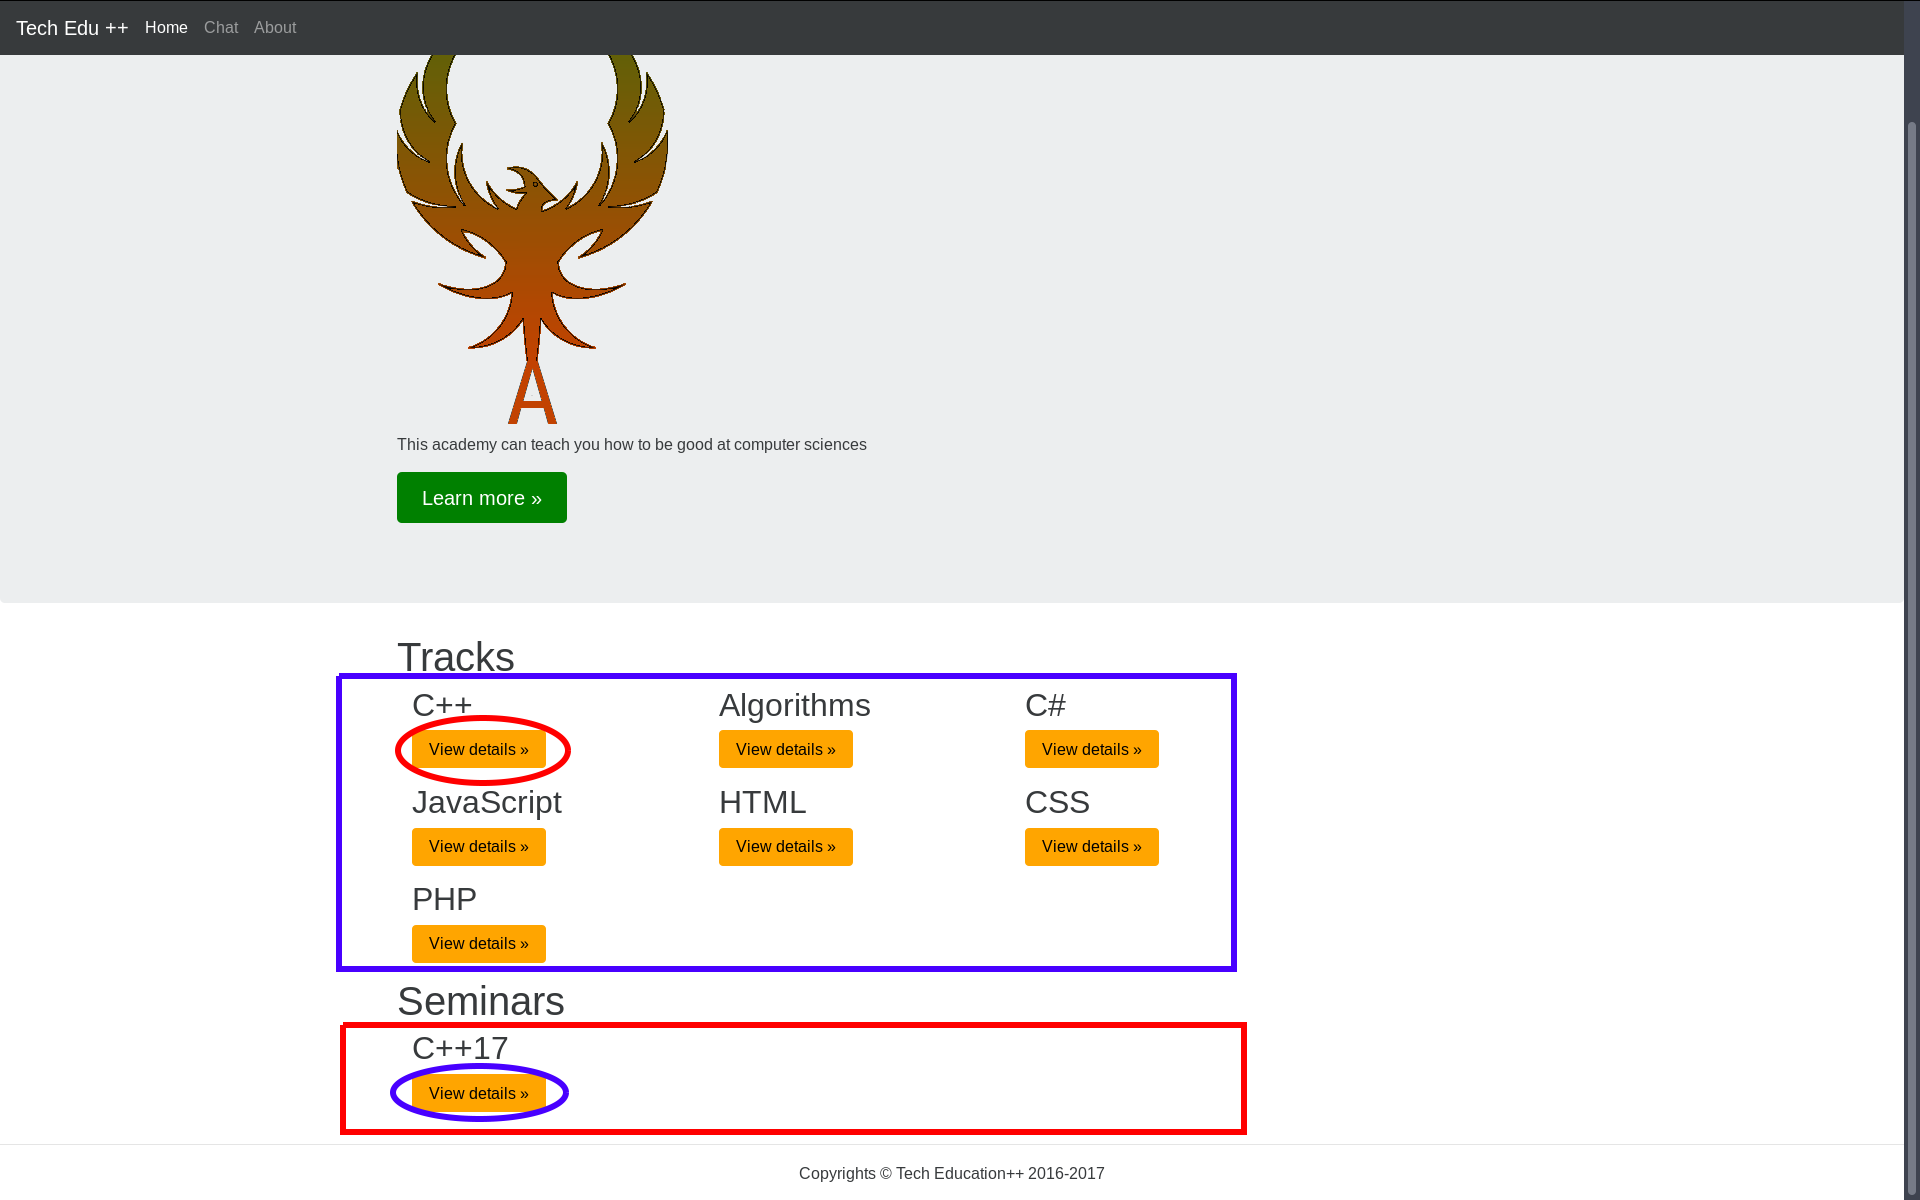
\includegraphics[width=0.8\textwidth]{track_view.png}\\
	\\При преглед на курс има множество озаглавени уроци и когато се кликне бутона „View details »“ ще се появи вграден прозорец със съответното видео.\\
	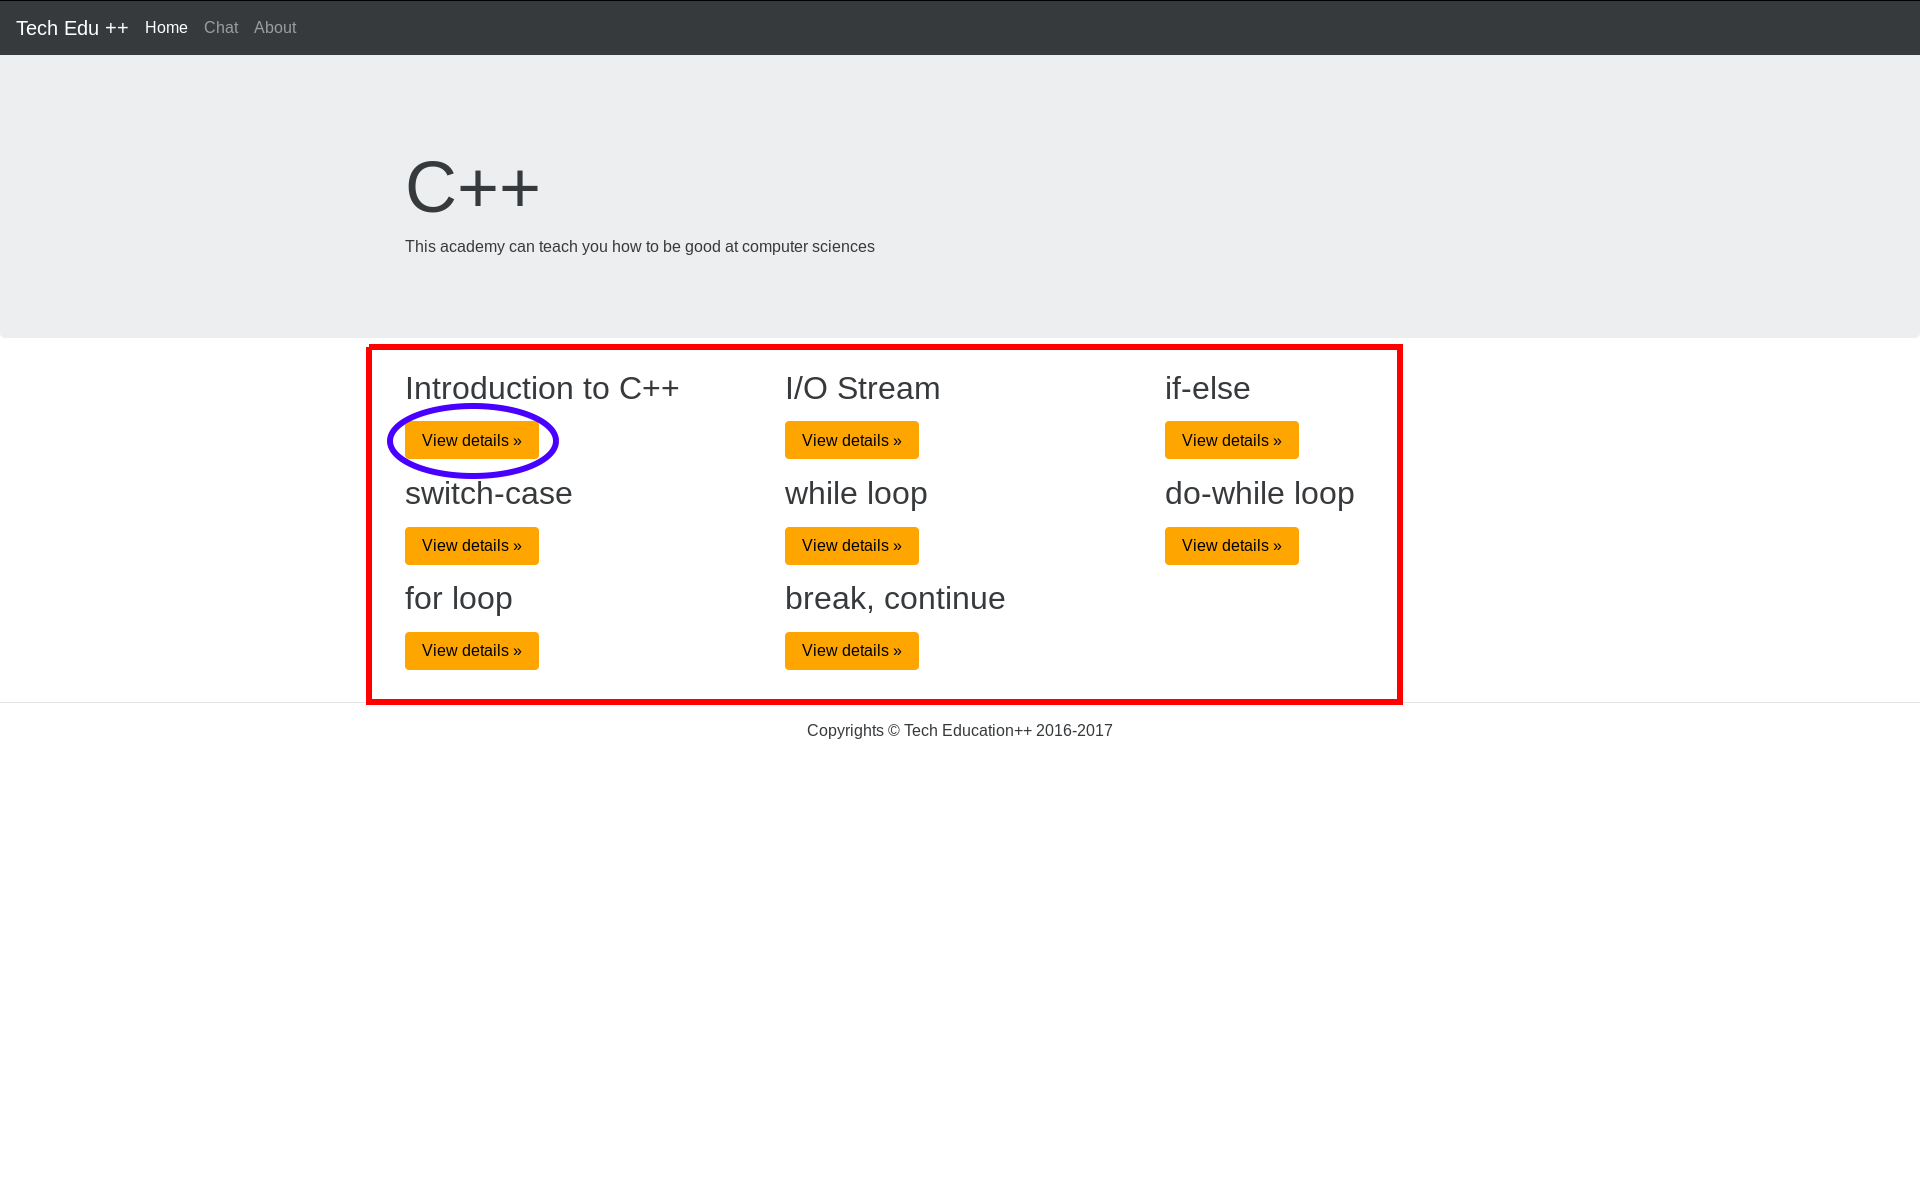
\includegraphics[width=1\textwidth]{view_details.png}\\
	\\За да се прегледа съответния видео урок, трябва да се натисне бутона „View details »“ за съответния урок и се появява вграден прозорец със съответното видео.\\
	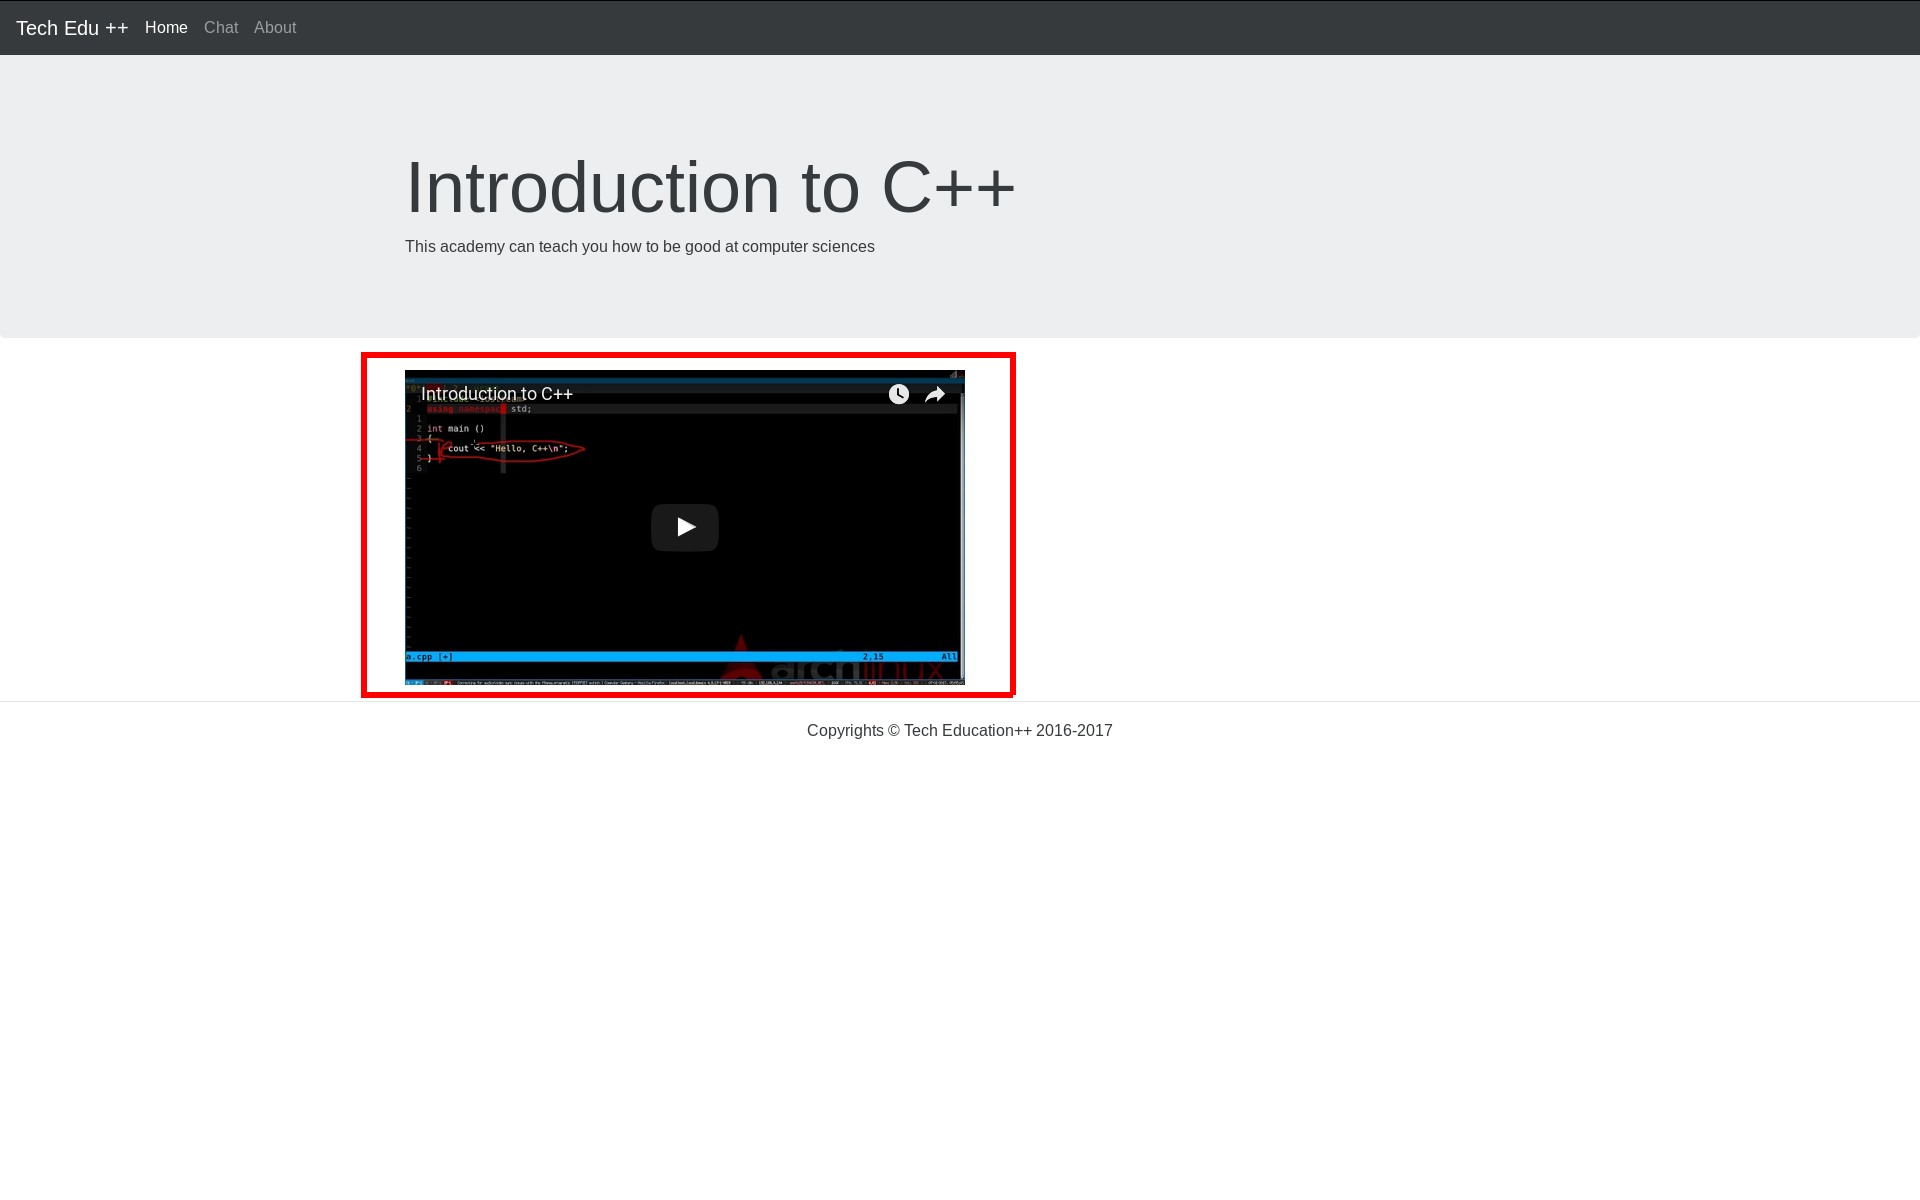
\includegraphics[width=0.75\textwidth]{track_video.png}\\
	\\При преглед на семинар директно ще се появи вграден прозорец със съответния видео урок.\\
	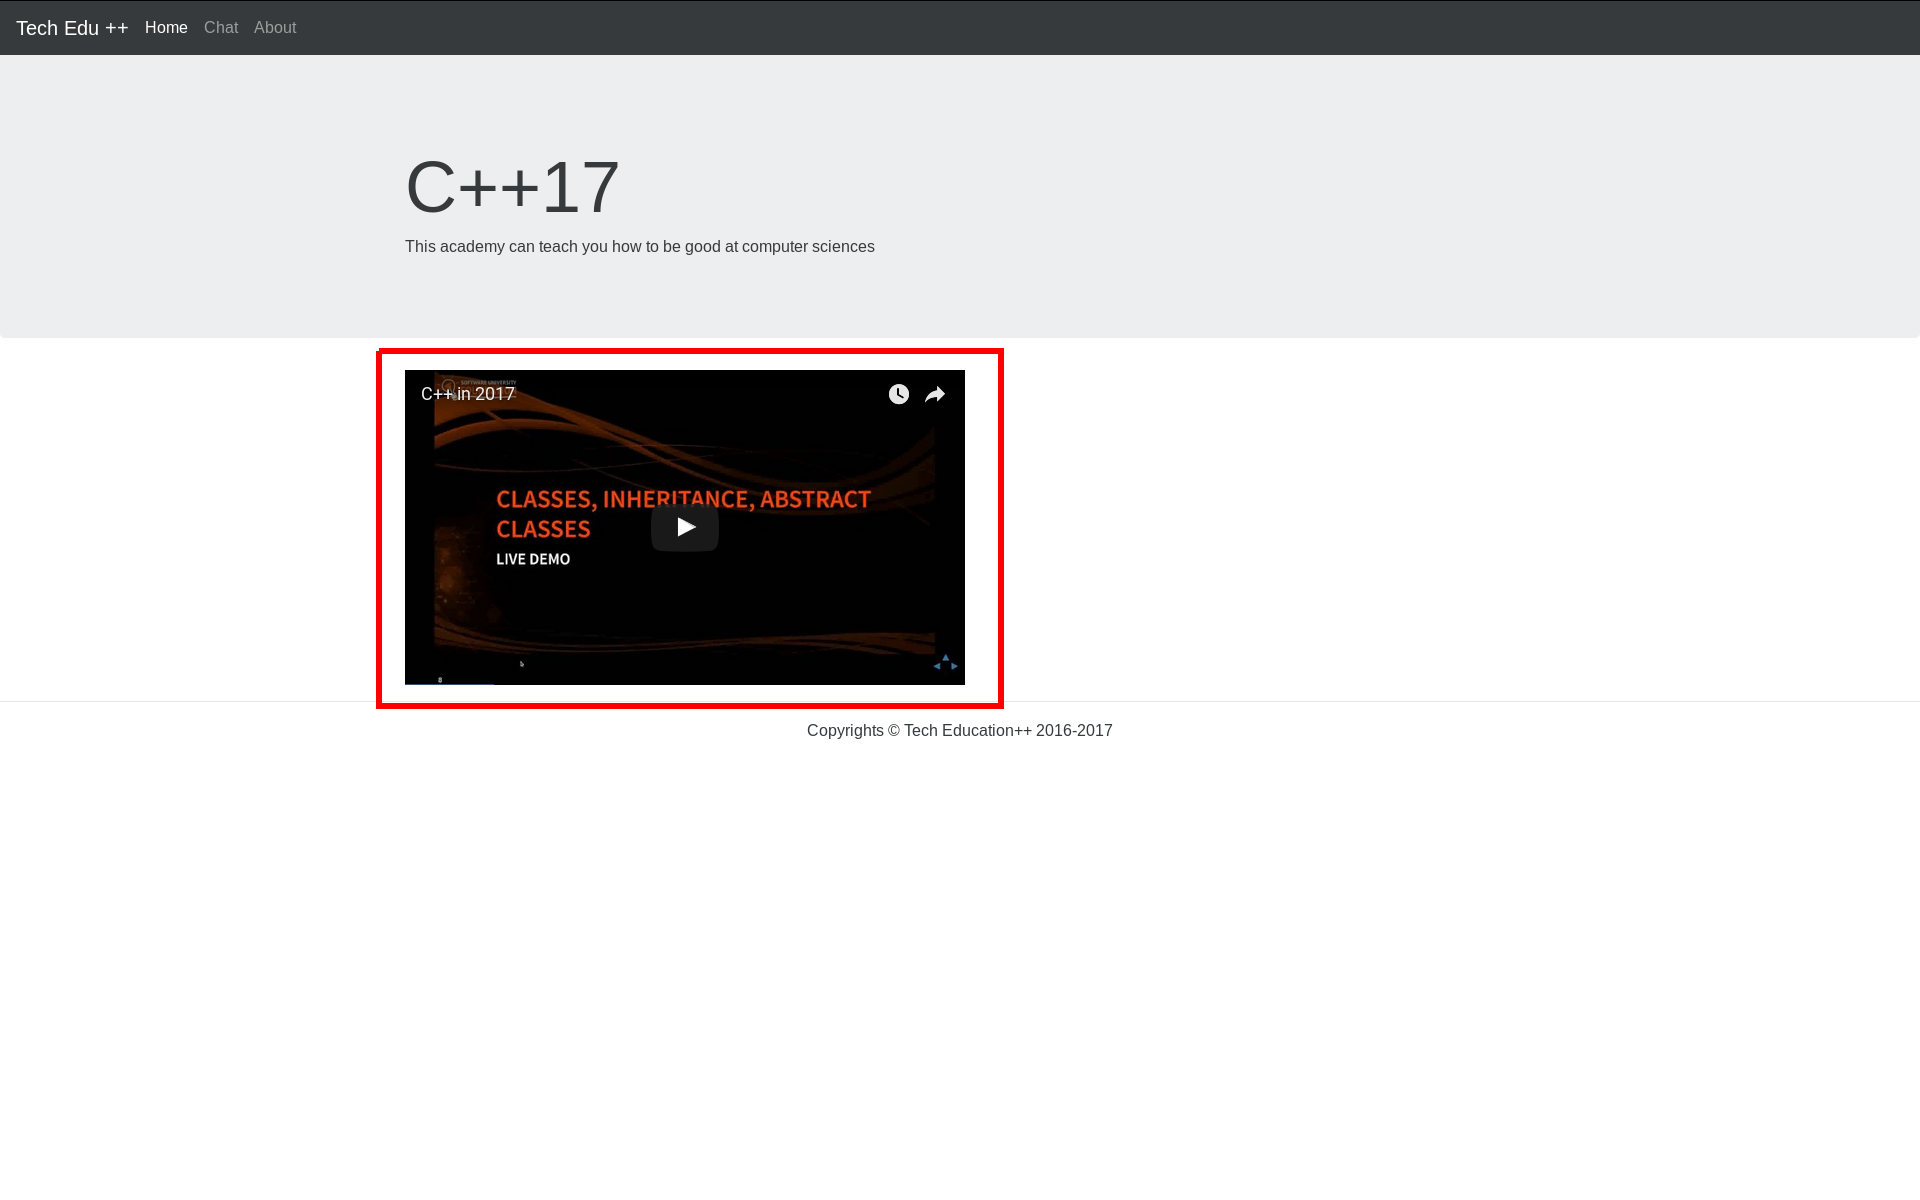
\includegraphics[width=1\textwidth]{seminar_video.png}\\
	\section{Заключение}
	Резултатът до момента е създаването на основата на образователно-информационна платформа, която да може да се усъвършенства и обновява, за да бъде в крак с времето и технологиите. 
	Бъдещото развитие включва:
	\begin{itemize}
		\item добавяне на система от знания по други актуални програмни езици като JavaScript, TypeScript, Java, Python и т.н.
		\item популяризиране на проекта сред учащите се
		\item разширяване на кръга от контакти с действащи фирми
	\end{itemize}
\end{document}
